\section{\tool{} Leakage Definition}
In the section, we discuss how \tool{} quantifies the amount of
leaked information. \tool{} is a dynamic-based approach to 
quantify the information leakage. We will first introduce 
the limitation of existing quantification metrics. After
that, we introduce the abstract and notation for the paper 
and propose our method.

\subsection{Problem Setting}
Existing static-based side-channel quantification works~\cite{182946,Wichelmann:2018:MFF:3274694.3274741 } define information leakage
using max entropy or Shannon entropy. These definitions provide a strong security guarantee
when trying to prove a program is secure enough if zero bit of information is leaked 
reported by their approaches. However, it is useless if the tool report the program leaks
some information. Moreover, those metrics does not apply to static method.


\begin{figure}[h!]
    \centering
\begin{lstlisting}[xleftmargin=.03\textwidth,xrightmargin=.01\textwidth]
uint8_t password = input();
if(password == 0x1b){
    pass();     //branch 1
}else{
    fail();     //branch 2
}
\end{lstlisting}
\caption{A dummy password checker}
\label{figure:password checker}
\end{figure}

We consider the above dummy password checker~\ref{figure:password checker}.
The program will take a 8 bit number as the input and check if the input is the
correct password. 
If an attacker knows the
code executes branch $\{{1\}}$ by side-channel attacks, he can infer the password equals to 0x1b,
in which case the attacker can fully retrieve the password.
Therefore, the total information leakage should be 8 bits, which equals to the size
of the sensitive input. 

However, previous static-based approach can not precisely reflect the sensitivity of the leakage.
According to the definition of Shannon entropy, the leakage will be $\frac{1}{256}*\log_{2}\frac{1}{256} + 
\frac{255}{256} *\log_{2}\frac{255}{256}= 0.24$ bits. Because the program has two branches, tools
based on max-entropy will report the code has $\log_2{2} = 1$ bit leakage.

Both approaches fail to tell how 
much information is leaked during the execution precisely.

The problem with the existing methods is that they are static-based and the 
input values are neglected by the previous definition. 
They assume the attacker runs the program multiple times with many different sensitive 
information as the input. Both Shannon entropy and max entropy give an ``average" 
estimate of the information leakage. However, it is not the typical scenario for an adversary to 
launch a side-channel attack. When a side-channel attack happens, the adversary wants 
to retrieve the sensitive information, in which case the sensitive information is fixed (e.g. AES keys). 
The adversary will run the attack over and over again and guess the value bit by bit. Like the 
previous example, the existing static method does not work well in those situations.
We want to have a theory for dynamic analysis that if the theory says 
an attack leaks $x$ bits of secret information from side-channel vulnerabilities,
then $x$ should be useful in estimating the sensitive level of side-channels.
However, the above method all fails in the real attack model.
\begin{figure}
  \centering
   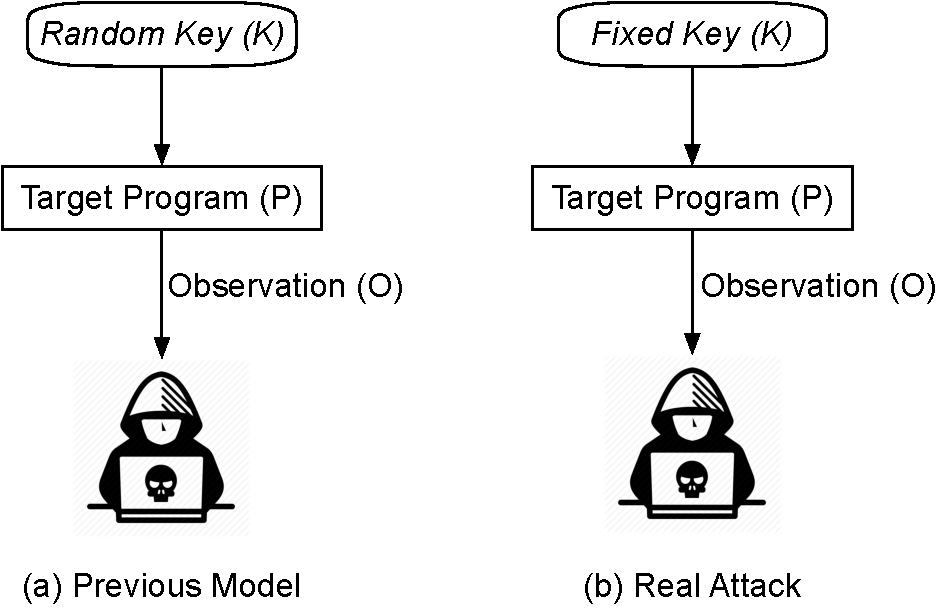
\includegraphics[width=.9\columnwidth]{./figures/RA.pdf}
   \caption{The gap between the real attack and previous model}
\end{figure}


\subsection{Notations}
In the section, we give the necessary definitions and notations for dealing 
with programs and side-channels. We use capital letters (e.g., $S$) to represent 
the set. $|S|$ represents the size of set $S$. We use corresponding small letters
to represents one element in the set (e.g., $s \in S$).

We assume the program ($\beta$) has $K$ as the sensitive input. 
$K$ should be a finite set of keys. The program also takes known messages $M$ as the input. 
The model applies to most of the cryptosystems. For example,
during the AES encryption, $\beta$ is the encryption function. $K$ is AES key and
$M$ is the message to be encrypted. During the execution, an adversary may have some observations ($O$) from the program. Examples of those observations
include timing, CPU usages, and Electromagnetic signals (EM). For the paper, we
consider the secret-dependent control-flows and secret-dependent memory accesses
as the observations.

With the above definitions, we have the following mapping between $\beta$, $K$, $M$, and $O$:

\begin{displaymath}
    \beta(K, M) \rightarrow	O
\end{displaymath}

An adversary does not have access to $K$, but he should know $\beta$, $M$, and $O$. 
For one execution of a deterministic program, once $k \in K$ and $m \in M$ are fixed, the 
observation ($o \in O$) is also determined. As an attacker, he knows $\beta$, $o$, 
and $m$. The attacker wants to infer value of $k$. We use $K^o$ to denote the set of
$k$ that still produces the same observations:

\begin{displaymath}
    K^o = \{ k \in K \, |\, \beta(k, m) \rightarrow o\}
\end{displaymath}
The problem of quantifying the amount of leaked information can be transferred into the
following question: 

How much uncertainty of $K$ can be reduced if an attacker knows $\beta$, $m$, and $o$?  
 
\subsection{Theoretical Analysis}
In information theory, the mutual information (MI) of is a measure of the mutual dependence 
between the two variables. Here we use MI to describe the leakage between $K$ and $O$, 
which is defined as:

\begin{equation} \label{eq:1}
    I(K;O) = \sum_{k_i {\in} K}{\sum_{o_j {\in} O}{p(k_i, o_j)\log_2\frac{p(k_i, o_j)}{p(k_i)p(o_j)}}}
\end{equation}

where $P(k_i, o_i)$ is the joint discrete distribution of $K$ and $O$.
Alternatively, the mutual information can also be equivalently expressed as:
\begin{equation} \label{eq:2}
    I(K;O) = H(K) - H(K|O)
\end{equation}

$H(K|O)$ is the entropy of $K$ conditioned on $O$. It quantifies the uncertainty of $K$
given the value of $O$. In other word, the conditional entropy $H(K|O)$ marks the 
uncertainty about $K$ after the adversary has gained some observations ($O$). 
\begin{equation}
    H(K|O) = - \sum_{o_j {\in} O} {p(o_j) \sum_{k_i {\in} K}{p(k_i|o_j)\log_2p(k_i|o_j)}}
\end{equation}

In the project, we hope to give a very precise definition of information leakages. 
Suppose an attacker run the target program multiple times with one fixed input, we
want to know how much information he can infer by observing the memory access patterns ($o$).
We come to the simple slogan ~\cite{10.1007/978-3-642-00596-1_21} %% where the information
%% leakage equals:
%% \textbf{Initial uncertainty - remaining uncertainty}
that
\begin{align*}
 & \mathit{Information\ leakage} = \\
 & ~~~~~~ \mathit{Initial\ uncertainty} - \mathit{Remaining\ uncertainty}. 
\end{align*}

Now we come compare the equation~\ref{eq:2} with the above slogan, we will
find $H(K)$ is the $\mathit{Initial\ uncertainty}$ and $H(K|O)$ is
$\mathit{Remaining\ uncertainty}$. During a side-channel attack, 
the observation ($o$) is known.  We have $H(K|O) = H(K|o)$.

Therefore, we define the amount of leaked information as 
\begin{displaymath}
    Leakage = H(K;o) = H(K) - H(K|o)
\end{displaymath}

For a program ($\beta$) without knowing any domain information, any sensitive
input should appear equally. Therefore, for any $k \in K$, $p(k) = \frac{1}{|K|}$.
So we have 
$$H(K) = \sum_{k {\in} K}\frac{1}{|K|}log_2{|K|} = log_2{|K|}$$
For any $k' \in K - K^o$, $p(k'|o) = 0$. We can get the following equation:
\begin{align*}
H(K;o) &= - \sum_{k {\in} K^o}{p(k|o)\log_2p(k|o)} 
          - \sum_{k` {\in} (K - K^o)}{p(k'|o)\log_2p(k'|o)}\\
       &= \sum_{k {\in} K^o}\frac{1}{|K^o|}log_2{|K^o|}\\
       &= log_2{|K^o|}
\end{align*}

\newtheorem{mydef}{Definition}

\begin{mydef}
\label{def}
Given a program $\beta$ with the input set $K$, 
an adversary has the observation $o$ when the input $k{\in}\hat{K}$. 
We denote it as
$$\beta(K^o, m) \rightarrow	o$$

The leakage $L_{\beta(k)\rightarrow o}$ based on the observation ($o$) is
    $$L_{\beta(k)\rightarrow o} = \log_2{|K|} - \log_2{|K^o|}$$
\end{mydef}

With the new definition, if the attacker observes that the code~\ref{figure:password checker} runs the branch 1, 
then the $K^{o^{1}} = \{\mathrm{0x1b}\}$. Therefore, the information leakage $L_{P(k)=o^{1}} = \log_2{256} - \log_2{1} = 8$
bits, which means the key is totally leaked. If the attacker observes the code runs branch2, the leaked information is 
$L_{P(k)=o^{2}} = \log_2{256} - \log_2{255} = 0$ bit.


We can also calculate the leaked information
from the sample code~\ref{background::side-channel}. As the size of input 
sensitive information is usually public. The problem of quantifying the
leaked information has been transferred into the problem of estimating
the size of $|K^o|$.

\begin{table}[ht]
    \centering

 %  \resizebox{.8\columnwidth}{!}{

\begin{tabular}{l|cccc}
    \hline
%Observation (o)     & $\emptyset$ & ${\{1\}}$ & ${\{2\}}$ & ${\{1, 2\}}$ \\ \hline
%Number of Solutions &  32876 & 20 & 32634 & 16 \\ \hline
%Possibility (p)     & 0.5016 & 0.0003 & 0.4980  & 0.0002   \\
Observation ($o$)  & $\emptyset$ & ${\{1\}}$ & ${\{2\}}$ & ${\{1, 2\}}$ \\ \hline
Number of Solutions &  32876 & 20 & 32634 & 16 \\ \hline
Leaked Information (bits)     & 1.0 & 11.7 & 1.0  & 12.0   \\
    \hline
\end{tabular}
%    }
\caption{The distribution of observation}
\label{shtable}
\end{table}

